
\chapter{Vorgehensweise}

\section{Datengewinnung}

Die Trainingsdaten wurden mit Hilfe des DuckieTown-Simulator erstellt.

\section{Netzwerkarchitektur}

Unsere Netzwerkarchitektur besteht aus einer Normalisierungsschicht (normalization layer), fünf Faltunsschichten (convolutional layers) und drei Fully-Connected-Schichten (fully connected layers). Das Netzwerk nimmt das  Kamerabild des DuckieBots als Eingabe entgegen, wobei das obere drittel des Kamerabildes entfernt wurde. Eine schematsche Darstellung der Netzarchitektur ist in Abbildung \ref{network-architecture} dargestellt. \\

Die Normalisierungsschicht des Netzwerks kümmert sich um die Normalisierung des Eingabebildes, wodruch die GPU-Verabeitung beschleunigt wird. \\

Die Faltungsschichten kümmern sich um die Extraktion von Bildmerkmalen. Die ersten drei Faltungsschichten nutzen dabei einen 5x5 Kernel mit einer 2x2 Schrittbreite (stride) und die letzen beiden einen 3x3 Kernel mit einer 1x1-Schrittbreite. \\

Nach den Faltungsschichten folgen drei Fully-Connected-Schichten die uns schlussendlich die geschätzte Distanz $d$ und geschätzte Orientierung $\Theta$ liefern.


\begin{figure}[H]
	\centering
	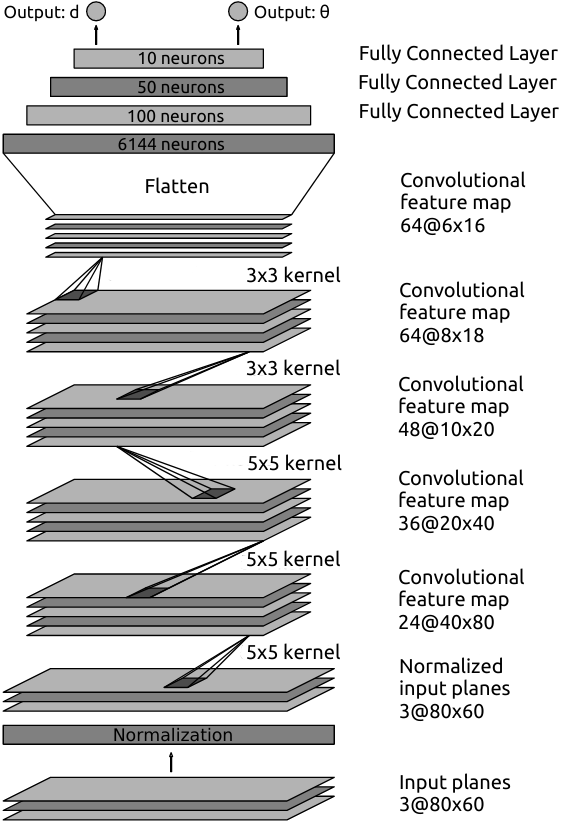
\includegraphics[width=0.75\textwidth]{kapitel4/images/network_architecture.png}
	\caption{Schematische Darstellung der Netzwerkarchitektur}
	\label{network-architecture}
	\vspace{0.2cm}
	\quelle\url{https://d3i71xaburhd42.cloudfront.net/0e3cc46583217ec81e87045a4f9ae3478a008227/5-Figure4-1.png}
\end{figure}




